% !TEX root = ../notes_unsupervisedlearning.tex
% Chapter 12: Interactive and Imitation Learning
%%%%%%%%%%%%%%%%%%%%%%%%%%%%%%%%%%%%%%%%%%%%%%%%%%%%%%%%%%%%%%%%%%%%%%

\chapter{Interactive and Imitation Learning}\index{Active Learning}\index{Imitation Learning}\index{Behavior Cloning}
\newthought{Humans correct, query, and demonstrate.}

%═══════════════════════════════════════════════════════════════════════
% BLOCK 1: INTRODUCTION
%═══════════════════════════════════════════════════════════════════════

\section{The Why}\index{active learning}\index{imitation learning}\index{behavior cloning}

\marginnote{\newthought{Demonstration.}\index{demonstration} A trajectory of state-action pairs
recorded from a competent actor, usually a human, sometimes a scripted controller.
A demonstration carries more information per second of human time than a scalar reward,
because every action labels a state.}

\newthought{In the previous chapter} an agent learned to act from a scalar reward,
and Bellman decomposition reduced the long-horizon credit-assignment problem to local updates.
The decomposition is correct, but it does not make the reward less sparse,
and across long horizons the agent burns millions of steps before any informative signal arrives.
A human watching the same agent could correct one wrong move, demonstrate the right one,
or rank two trajectories in seconds, each input a silver bullet that carries more information
per second of human time than any per-example label could,
and the methods of this chapter are built to absorb that few-shot supervision.

\marginnote{\newthought{Annotation costs.}\index{annotation cost} Annotation cost scales with the task.
A radiologist contouring a tumour costs orders of magnitude more per label
than a crowd worker tagging a cat,
and a human teleoperating a robot arm costs more still.
The structural problem is to spend that budget where it changes the model the most.}

\marginnote{\newthought{RL doesn't work yet.}\index{reinforcement learning} Alex Irpan's much-cited essay catalogues the ways deep
reinforcement learning fails in practice: sample inefficiency, brittle hyperparameters,
reward hacking, exploration that gives up, and policies that fail to generalise.
Worth reading before convincing yourself that scalar-reward RL is the answer to your problem.\\
\url{https://www.alexirpan.com/2018/02/14/rl-hard.html}}

\newthought{Reward learning is sample-inefficient,} reward functions are hard to specify,
and exploration through random action wastes the most expensive part of the loop, the human.
Interactive and imitation learning sidestep these failure modes
by treating human queries, demonstrations, and preferences as first-class supervision.

\marginnote{\newthought{Acquisition function.}\index{acquisition function} The function that ranks unlabelled
examples by anticipated information gain, the central object of any active-learning pipeline.
Uncertainty sampling, query-by-committee, and expected model change are three families of acquisition function,
and the choice between them depends on whether the model is well calibrated.}

\newthought{Active learning.}\index{active learning}
The learner holds a pool of unlabelled examples and a budget of queries,
and it asks the annotator only for the labels that move the model the most.
Uncertainty sampling queries the points where the predictive distribution is closest to uniform,
query by committee trains an ensemble and queries where its members disagree~\cite{Settles2012ActiveLearning},
and the choice of strategy depends on whether the model is well calibrated.

\newthought{Batch active learning.}\index{batch active learning}
Annotators label in batches, and querying $B$ near-duplicate uncertain points wastes the budget.
Batch strategies score a set rather than a point, trading information against diversity
through greedy selection with a coverage constraint, core-set selection,
or BatchBALD-style joint information gain.

\marginnote{\newthought{ALVINN.}\index{ALVINN} The Autonomous Land Vehicle In a Neural Network learned to steer
from a windshield camera by behaviour cloning from a human driver~\cite{Pomerleau1991ALVINN}.
The same paper that demonstrated the recipe also surfaced its central failure mode:
small steering errors push the car towards lane edges the human never visited,
and the supervision the network was trained on no longer applies.}

\newthought{Behaviour cloning.}\index{behavior cloning}
Treat expert state-action pairs as a supervised dataset and fit a policy by maximum likelihood~\cite{Pomerleau1991ALVINN}.
The recipe is simple and it scales, but the learner is trained on the expert's state distribution
while it acts on its own, so small errors push it off-distribution and the policy compounds them
into large failures, the covariate shift problem.

\marginnote{\newthought{Covariate shift.}\index{covariate shift} The mismatch between the distribution of states
the learner saw at training time, the expert's, and the distribution it sees at deployment, its own.
Behaviour cloning trains on the former and tests on the latter, and the supervision the network was fitted
on no longer applies once the learner steps outside the expert's tube of trajectories.}

\newthought{DAgger.}\index{DAgger}
Dataset Aggregation closes that loop by rolling out the current learner,
querying the expert for the correct action at every state the learner visits,
and retraining on the aggregated data~\cite{Ross2011DAgger}.
The expert now labels the learner's own state distribution,
which is exactly the distribution the deployed policy will face.

\newthought{Inverse reinforcement learning.}\index{inverse reinforcement learning}
Sometimes copying actions is the wrong target, because the same action means different things
in different states, and the reward function transfers across embodiments and environments where the policy does not.
IRL recovers the reward that explains the expert, and Maximum Entropy IRL\index{MaxEnt IRL} resolves the ambiguity
by choosing the reward under which expert trajectories are maximally likely
without committing to assumptions the data does not justify~\cite{Ziebart2008MaxEntIRL}.

\newthought{Generative adversarial imitation learning.}\index{GAIL}
GAIL skips the explicit reward and trains a discriminator to separate expert from learner trajectories,
while the policy is trained to fool it~\cite{Ho2016GAIL}.
The adversarial signal plays the role of a reward,
and the method inherits the scalability of policy gradient methods without the brittleness of hand-designed rewards.

\marginnote{\newthought{Reward model.}\index{reward model} A model trained on pairwise human comparisons
that scores candidate outputs. RLHF uses one as a stand-in for the explicit reward function~\cite{Christiano2017Preferences},
allowing PPO to optimise against learned human preference instead of a hand-written reward,
and inheriting the calibration biases of the labellers who wrote those preferences.}

\newthought{Reinforcement learning from human feedback.}\index{RLHF}
At scale, the cheapest human signal is a preference between two outputs.
Christiano and colleagues showed that a reward model fit to pairwise preferences
suffices to align an RL agent with hard-to-specify objectives~\cite{Christiano2017Preferences},
and InstructGPT extended the recipe to language models through supervised fine-tuning,
reward modelling, and PPO optimisation~\cite{Ouyang2022InstructGPT}.
Direct Preference Optimisation\index{DPO} later showed that the reward model can be folded into the policy loss itself,
removing the RL stage~\cite{Rafailov2023DPO}.

\newthought{In order to move from passive data consumption to efficient human-guided learning}
we have good reason to find ways to,
\begin{itemize}
    \item select the few examples whose labels move the model the most,
    so that an annotation budget buys the largest possible improvement.
    \item learn policies from expert demonstrations by maximum likelihood,
    while controlling the covariate shift that compounding errors create when the learner leaves the expert's state distribution.
    \item close the demonstration loop by querying the expert at the states the learner actually visits,
    so the supervision tracks the deployed policy's distribution rather than the expert's.
    \item recover the reward function that explains expert behaviour,
    so that the learned objective transfers to environments and embodiments the demonstrations did not cover.
    \item turn pairwise human preferences into a training signal for systems
    whose desired behaviour is too complex to specify by hand,
    with or without an explicit RL stage in the optimisation loop.
\end{itemize}

\newthought{The fundamental question} this chapter answers is how to spend a fixed amount of human attention
so that each query, demonstration, or preference teaches the model as much as possible,
and how to keep the resulting policy robust once the human steps away.

\newpage

\iffalse
\subsection{Hands On Experience}

\begin{marginfigure}
\begin{tikzpicture}[scale=0.7]
    \begin{axis}[
        xlabel={$x_1$}, ylabel={$x_2$},
        xmin=0, xmax=10, ymin=0, ymax=10,
        width=\textwidth, height=\textwidth,
        axis line style={draw=none},
        tick style={black, thin},
        tick align=outside, tick pos=left,
        xtick={2,4,6,8}, ytick={2,4,6,8},
        xticklabel style={font=\tiny},
        yticklabel style={font=\tiny},
    ]
    % Decision boundary
    \addplot[black, thick, domain=0:10] {5};
    % Labeled points
    \addplot[only marks, mark=*, mark size=2pt, black] coordinates {(2,2) (3,1)};
    \addplot[only marks, mark=*, mark size=2pt, black!55] coordinates {(8,8) (7,9)};
    % Unlabeled near boundary
    \addplot[only marks, mark=o, mark size=2pt, black, thick] coordinates {
        (4,5.2) (5,4.8) (6,5.1)
    };
    % Unlabeled far from boundary
    \addplot[only marks, mark=o, mark size=1.5pt, black!30] coordinates {
        (1,1) (9,9) (2,8) (8,2)
    };
    \end{axis}
\end{tikzpicture}
\caption{Active learning: query points near the decision boundary, where uncertainty is highest.}
\label{fig:active_learning_intro}
\end{marginfigure}

You have a budget to label 5 examples. Given the current decision boundary, which points would be most valuable to label?

Points near the boundary are uncertain; labelling them helps refine the boundary. Points far from the boundary are already well-classified.

\newthought{The Learning Objectives} of this lecture:
\begin{itemize}
    \item Implement active learning with uncertainty, disagreement, and diversity sampling, and choose the appropriate strategy for a given budget.
    \item Apply behaviour cloning and DAgger for learning from demonstrations, and explain why naive cloning suffers from compounding errors.
    \item Describe inverse reinforcement learning and RLHF as methods that recover or align reward functions from human behaviour.
\end{itemize}

%═══════════════════════════════════════════════════════════════════════
% BLOCK 2: MAIN THEORY
%═══════════════════════════════════════════════════════════════════════

\newpage
\section{Active Learning}\index{active learning}

\marginnote{Choose which examples to label for maximum information gain~\cite{Settles2012ActiveLearning}.}

\subsection{Setting}

\newthought{The active learning setup:} a pool $\mathcal{U}$ of unlabelled examples, a budget $B$ for labelling queries, and the goal of maximising model performance with $B$ labels.

\subsection{Query Strategies}

\newthought{Uncertainty sampling}\index{uncertainty sampling} queries examples where the model is most uncertain:

\begin{equation}
    x^* = \arg\max_{x \in \mathcal{U}} U(f(x))
\end{equation}

Uncertainty measures include entropy $H(p) = -\sum_k p_k \log p_k$, margin $1 - (p_1 - p_2)$ where $p_1 > p_2$ are the top probabilities, and least confidence $1 - \max_k p_k$.

\newthought{Query-by-committee}\index{query-by-committee} trains an ensemble and queries where members disagree:
\begin{equation}
    x^* = \arg\max_{x \in \mathcal{U}} \text{Disagreement}(\{f_1(x), \ldots, f_M(x)\})
\end{equation}

\newthought{Diversity sampling}\index{diversity sampling} ensures queried points cover the input space:
\begin{equation}
    x^* = \arg\max_{x \in \mathcal{U}} \min_{x' \in \mathcal{L}} d(x, x')
\end{equation}

\begin{figure}
\centering
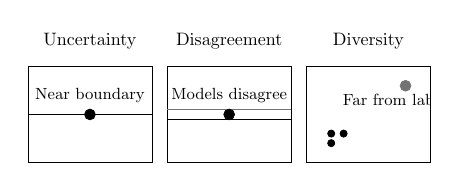
\begin{tikzpicture}[scale=0.65]
    % Uncertainty
    \begin{axis}[
        name=unc,
        title={Uncertainty},
        xmin=0, xmax=10, ymin=0, ymax=10,
        width=0.33\textwidth, ticks=none,
    ]
    \addplot[black, thick, domain=0:10] {5};
    \addplot[only marks, mark=*, mark size=3pt, black] coordinates {(5,5)};
    \node at (axis cs:5,7) {\small Near boundary};
    \end{axis}

    % Disagreement
    \begin{axis}[
        at={(unc.east)}, anchor=west, xshift=0.3cm,
        name=dis,
        title={Disagreement},
        xmin=0, xmax=10, ymin=0, ymax=10,
        width=0.33\textwidth, ticks=none,
    ]
    \addplot[black, thick, domain=0:10] {4.5};
    \addplot[black!55, thick, domain=0:10] {5.5};
    \addplot[only marks, mark=*, mark size=3pt, black] coordinates {(5,5)};
    \node at (axis cs:5,7) {\small Models disagree};
    \end{axis}

    % Diversity
    \begin{axis}[
        at={(dis.east)}, anchor=west, xshift=0.3cm,
        title={Diversity},
        xmin=0, xmax=10, ymin=0, ymax=10,
        width=0.33\textwidth, ticks=none,
    ]
    \addplot[only marks, mark=*, mark size=2pt, black] coordinates {
        (2,2) (3,3) (2,3)
    };
    \addplot[only marks, mark=*, mark size=3pt, black!55] coordinates {(8,8)};
    \node at (axis cs:8,6.5) {\small Far from labelled};
    \end{axis}
\end{tikzpicture}
\caption{Three query strategies select different points.}
\label{fig:query_strategies}
\end{figure}

\subsection{Batch Active Learning}\index{batch active learning}

\newthought{Querying multiple points at once} avoids redundancy:
\begin{equation}
    S^* = \arg\max_{S \subset \mathcal{U}, |S|=B} \text{BatchUtility}(S)
\end{equation}

Approaches include greedy selection with a diversity constraint, core-set selection, and BatchBALD.


\section{Human-in-the-Loop Learning}

\marginnote{Humans provide continuous feedback during training.}

\newthought{Feedback types} range from direct labels and corrections to comparisons where the human indicates ``A is better than B'', rankings where the human orders examples by quality, and demonstrations where the human shows how to perform a task.

\newthought{When to query:} low confidence predictions, high disagreement among models, out-of-distribution inputs, and periodic sampling for monitoring.


\section{Behavior Cloning}\index{behavior cloning}

\marginnote{Supervised learning on state-action pairs from demonstrations~\cite{Pomerleau1991ALVINN}.}

\newthought{An expert provides demonstrations} $\mathcal{D} = \{(s_1, a_1), (s_2, a_2), \ldots\}$, and the policy $\pi_\theta$ is trained to predict actions:
\begin{equation}
    \theta^* = \arg\min_\theta \sum_{(s,a) \in \mathcal{D}} \mathcal{L}(\pi_\theta(s), a)
\end{equation}

\subsection{The Covariate Shift Problem}\index{covariate shift}

\begin{figure}
\centering
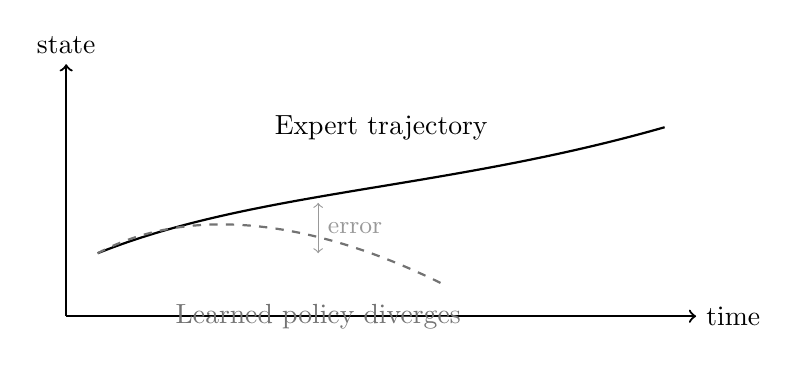
\begin{tikzpicture}[scale=0.8]
    \draw[->, thick] (0,0) -- (10,0) node[right] {time};
    \draw[->, thick] (0,0) -- (0,4) node[above] {state};

    % Expert trajectory
    \draw[black, thick] (0.5,1) .. controls (3,2) and (6,2) .. (9.5,3);
    \node at (5,3) {Expert trajectory};

    % Learned policy diverges
    \draw[black!55, thick, dashed] (0.5,1) .. controls (2,1.8) and (4,1.5) .. (6,0.5);
    \node[black!55] at (4,0) {Learned policy diverges};

    % Error compounds
    \draw[<->, black!40] (4,1.8) -- (4,1) node[midway, right] {\small error};
\end{tikzpicture}
\caption{Behaviour cloning: small errors compound, causing divergence from the expert trajectory.}
\label{fig:covariate_shift}
\end{figure}

\newthought{The problem:} the policy makes small errors that lead to states not seen in training. Performance degrades further. Errors compound exponentially.


\section{DAgger: Dataset Aggregation}\index{DAgger}

\marginnote{\newthought{DAgger.} Query the expert on the learner's state distribution~\cite{Ross2011DAgger}.}

\begin{algorithm}[H]
\caption{DAgger}
\begin{algorithmic}[1]
\State Initialize $\mathcal{D}$ with expert demonstrations
\State Train $\pi_1$ on $\mathcal{D}$
\For{$i = 1$ to $N$}
    \State Run $\pi_i$ to collect trajectories
    \State Query expert for actions at visited states
    \State Aggregate: $\mathcal{D} \gets \mathcal{D} \cup \mathcal{D}_i$
    \State Train $\pi_{i+1}$ on $\mathcal{D}$
\EndFor
\end{algorithmic}
\end{algorithm}

\newthought{The key insight:} train on states the learner actually visits, not just expert states.


\section{Inverse Reinforcement Learning}\index{inverse reinforcement learning}

\marginnote{Learn the reward function that explains expert behaviour~\cite{Ziebart2008MaxEntIRL}.}

\subsection{Motivation}

\newthought{Behaviour cloning copies actions} but does not capture why the expert acts that way. The reward function is more transferable than the policy, because it generalises to new situations.

\subsection{Maximum Entropy IRL}

\newthought{Find reward $r$} that makes the expert trajectory most likely:
\begin{equation}
    p(\tau | r) \propto \exp\left(\sum_t r(s_t, a_t)\right)
\end{equation}

Optimise:
\begin{equation}
    r^* = \arg\max_r \sum_{\tau \in \mathcal{D}_{\text{expert}}} \log p(\tau | r)
\end{equation}

\subsection{GAIL: Generative Adversarial Imitation Learning}\index{GAIL}

\marginnote{\newthought{GAIL.} Imitation as adversarial learning~\cite{Ho2016GAIL}.}

\newthought{GAIL} operates like a GAN but for trajectories: a discriminator distinguishes expert from learner trajectories, the policy tries to fool the discriminator, and no explicit reward learning is needed.


\section{Reinforcement from Human Feedback}\index{RLHF}

\marginnote{\newthought{RLHF.} How large language models learn from human preferences~\cite{Ouyang2022InstructGPT}.}

\begin{enumerate}
    \item Supervised fine-tuning: train on high-quality demonstrations
    \item Reward modelling: train a reward model on human comparisons
    \item RL fine-tuning: optimise the policy with PPO against the reward model
\end{enumerate}

\begin{figure}
\centering
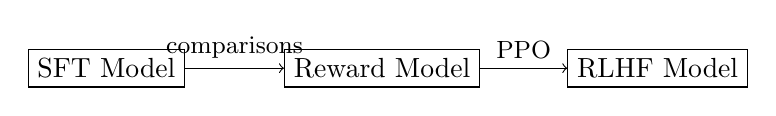
\begin{tikzpicture}[node distance=2cm]
    \node[draw, rectangle] (sft) {SFT Model};
    \node[draw, rectangle, right of=sft, xshift=1.5cm] (rm) {Reward Model};
    \node[draw, rectangle, right of=rm, xshift=1.5cm] (rlhf) {RLHF Model};

    \draw[->] (sft) -- node[above] {\small comparisons} (rm);
    \draw[->] (rm) -- node[above] {\small PPO} (rlhf);
\end{tikzpicture}
\caption{RLHF pipeline: SFT $\to$ Reward Model $\to$ RL Fine-tuning.}
\label{fig:rlhf_pipeline}
\end{figure}


%═══════════════════════════════════════════════════════════════════════
% BLOCK 3: STUDENT ACTIVATION
%═══════════════════════════════════════════════════════════════════════

\newpage
\section{Examples \& Exercises}

\subsection{Exercise 1: Active Learning Query}

Model outputs for 4 unlabelled points:
\begin{itemize}
    \item A: $p = [0.9, 0.1]$
    \item B: $p = [0.5, 0.5]$
    \item C: $p = [0.7, 0.3]$
    \item D: $p = [0.99, 0.01]$
\end{itemize}

Rank by uncertainty using entropy. Which would you query first?

\subsection{Exercise 2: Covariate Shift}

A self-driving car trained via behaviour cloning veers slightly right. Why does this get worse over time?

\subsection{Exercise 3: IRL vs.\ Behaviour Cloning}

When would you prefer IRL over behaviour cloning?


\fi

\section{Self-Reflection and Recap}\index{reflection}\index{recap}

\newthought{Self-Reflection} questions to guide your thinking:

\begin{itemize}
    \item Why does interactive supervision carry more information per second of human time than scalar reward, and what kinds of input, correction, demonstration, ranking, does this open up that scalar reward does not?
    \item Why does uncertainty sampling work when querying points where the predictive distribution is closest to uniform, and where does it break down when the model is poorly calibrated or when the boundary is in a region of low data density?
    \item What does query-by-committee buy on top of uncertainty sampling, and why does ensemble disagreement sometimes recover information that a single calibrated model misses?
    \item Why does batch active learning need a diversity term on top of an uncertainty term, and what would go wrong if you just queried the top-$B$ uncertain points from a single pass?
    \item Why is behaviour cloning trained on the expert's state distribution but evaluated on its own, and why does that mismatch turn small errors into compounding ones over a long trajectory?
    \item How does DAgger close the covariate-shift loop, and what does it cost in terms of expert availability and online query latency that the offline cloning recipe does not?
    \item Why is recovering the reward function with IRL more transferable than copying the actions with behaviour cloning, and what does Maximum Entropy IRL pin down that other formulations of the same problem leave ambiguous?
    \item How does GAIL turn imitation into adversarial learning, and what does this borrow from generative adversarial networks that the explicit-reward IRL methods do not?
    \item Why does RLHF train on pairwise preferences rather than absolute scores, and what does the reward model's job become once the human signal is reduced to a comparison?
    \item How does Direct Preference Optimisation eliminate the explicit RL stage that InstructGPT relied on, and what does folding the reward model into the policy loss buy in stability and simplicity?
    \item What goes wrong when the reward model used by RLHF is imperfect, and which failure modes (reward hacking, sycophancy, overoptimisation) does an imperfect reward model expose at scale?
    \item How would you combine active learning with imitation learning, querying the expert only at the states where the learner is most likely to fail rather than at uniformly sampled states?
\end{itemize}

\vspace{1.5em}

\newthought{Recap} of key concepts:

\begin{itemize}
    \item Active learning maximises information per label by querying points where the model is most uncertain, where ensemble members disagree, or where coverage of the input space is missing; batch strategies score a set rather than a point and trade information against diversity through greedy selection with a coverage constraint, core-set selection, or BatchBALD-style joint information gain so that an annotation budget buys the largest possible improvement.
    \item Behaviour cloning treats expert state-action pairs as a supervised dataset and fits a policy by maximum likelihood; the learner trains on the expert's state distribution while it acts on its own, and small errors push it off-distribution and compound, the covariate-shift problem, which DAgger closes by querying the expert at the states the learner actually visits and retraining on the aggregated data.
    \item Inverse reinforcement learning recovers the reward function that explains the expert rather than copying the actions themselves, and Maximum Entropy IRL resolves ambiguity by choosing the reward under which expert trajectories are maximally likely without committing to assumptions the data does not justify, while GAIL skips the explicit reward by training a discriminator to separate expert from learner trajectories with the policy trained to fool it.
    \item Reinforcement learning from human feedback turns the cheapest human signal at scale, a pairwise preference between two outputs, into a training signal: a reward model fit to preferences supplies the gradient for PPO in the InstructGPT recipe, and Direct Preference Optimisation later folded the reward model into the policy loss itself, removing the RL stage entirely while keeping the same supervision shape.
    \item Across active learning, behaviour cloning, IRL, GAIL, and RLHF, the unifying move is to spend a fixed budget of human attention where it teaches the model the most: queries near the boundary, demonstrations of the deployed state distribution, rewards that explain rather than copy, and preferences instead of absolute scores.
\end{itemize}

\vspace{2.5em}

\marginnote{\newthought{Teaser.} Interactive learning relies on human feedback for every loop.
What if the agent could imagine its own rollouts, query its own model, and reserve real interaction
only for the moments where imagination is no longer enough?}

\newthought{Interactive and imitation learning shift the cost of supervision onto the human.}
The methods are sample-efficient compared with scalar-reward RL,
but every demonstration, correction, and preference still spends a moment of human attention.
At scale, the budget that limits the loop is no longer the data, but the annotator.

\newthought{The next chapter introduces world models,}
where the agent learns a generative model of its environment and does most of its thinking in imagination,
trading expensive real interaction for cheap imagined rollouts.
Interactive learning derived its supervision from human queries and demonstrations;
world models derive theirs from the agent's own predicted dynamics.

\marginnote{\newthought{feedback}}
